\documentclass[12pt]{article}
\usepackage{graphicx}

\title{CarND Traffic Sign Classifier Project Writeup}
\author{Tiffany Huang}
\date{\today}

\begin{document}
\maketitle


\section{Traffic Sign Recognition Project}
This project consists on the following steps/tasks:
\begin{itemize}
\item{Load the data set}
\item {Explore, summarize, and visualize the data set.}
\item {Design, train, and test a model architecture}
\item {Use the model to make predictions on new images.}
\item {Analyze the softmax probabilities of the new images.}
\item {Summarize the results in a written report.}
\end{itemize}
My project code can be found here:

\section{Data Set Summary \& Exploration}
I used the \texttt{pandas} library to provide a summary of the data set. I found that the
\begin{itemize}
\item {Number of training examples = 34799}
\item {Number of validation examples = 4410}
\item {Number of testing examples = 12630}
\item {The shape of a traffic sign image was (26, 25)}
\item {Number of unique classes = 43}
\end{itemize}

\section{Exploratory Visualization of the Dataset}
To visualize the data, I used \texttt{matplotlib} to show the distribution of classes in the training, validation, and testing set. The histogram shows how many examples of each class exist in each dataset.
\begin{figure}[!h]
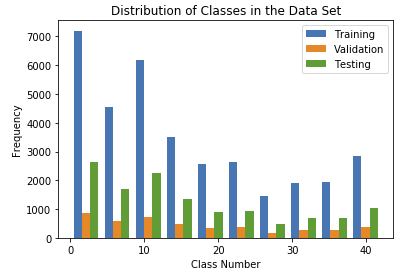
\includegraphics[scale=0.7]{writeup_images/distribution_classes.png}
\end{figure}

\section{Design and Test of a Model Architecture}
\subsection{Preprocessing}
The first step in my preprocessing was to crop the image so that only the traffic sign is in the image. This step removes the background of the image, which in most cases does not provide any useful information to determine what kind of sign is in the image. For instance, grass does not help to indicate a stop sign vs. a general caution sign. By removing the excess information-lacking data allows the CNN to focus on the important features in the image. To do the cropping correctly, I had to resize the image to the original size because the bounding boxes for the signs were given with respect to the original image size. After the cropping, I then resized the image to 32 $\times$ 32 $\times$ 3 because my CNN takes this size image as input. An example is shown below:
\begin{figure}[!h]
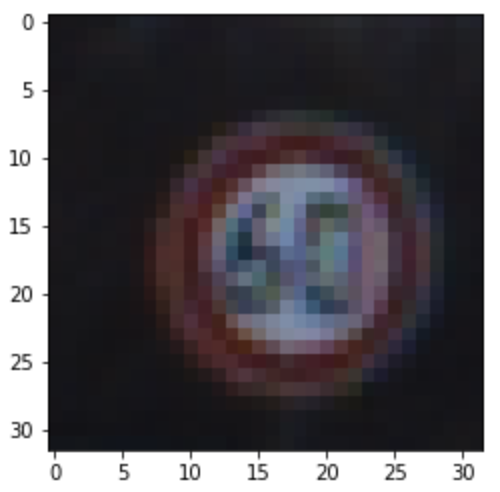
\includegraphics[scale = 0.5]{writeup_images/im1.png}
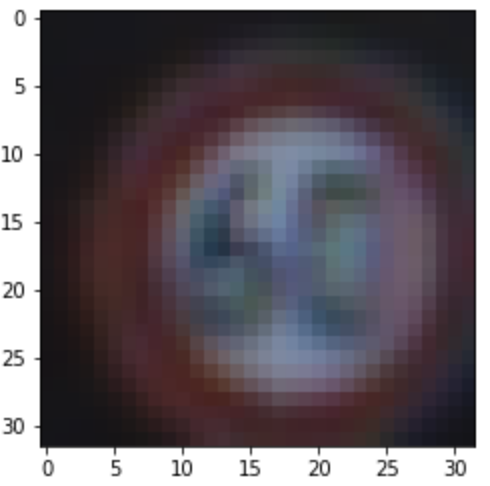
\includegraphics[scale = 0.5]{writeup_images/cropped.png}
\end{figure}

The next step was to normalize the image because different images were taken with different lighting, but different lighting should not affect the learned results. Thus, normalizing the image by subtracting the mean of the image and dividing by the standard deviation allows us to account for these environmental condition differences between images. An example of normalization is shown below:
\begin{figure}[!h]
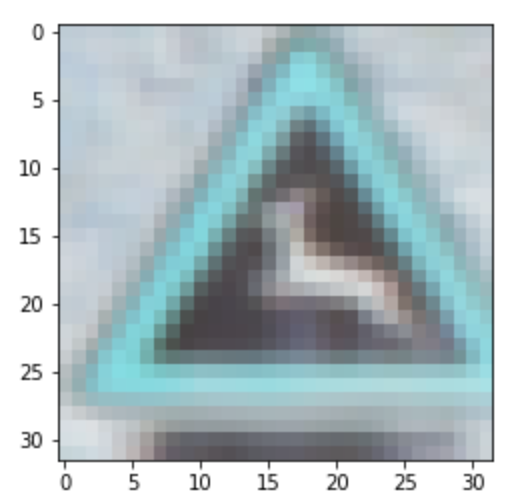
\includegraphics[scale = 0.5]{writeup_images/normalized.png}
\end{figure}

I chose not to convert the images to grayscale because I thought the colors of the traffic signs would be important features for the model to use for prediction.

\subsection{Final Model Architecture}
My final model consists of the following layers:
\begin{center}
\begin{tabular}{|c|c|}
\hline
\textbf{Layer} & \textbf{Description} \\
\hline
Input & 32 x 32 x 3 RGB Image \\
\hline
Convolutional & 1 x 1 stride, VALID padding, outputs 28 x 28 x 6 \\
\hline
Activation & ReLU \\
\hline
Max pooling & 2 x 2 window, 2 x 2 stride, SAME padding, outputs 14 x 14 x 6 \\
\hline
Convolutional & 1 x 1 stride, VALID padding, outputs 10 x 10 x 16 \\
\hline
Activation & ReLU \\
\hline
Max pooling & 2 x 2 window, 2 x 2 stride, SAME padding, outputs 5 x 5 x 16 \\
\hline
Flatten & Outputs 400 x 1 \\
\hline
Fully connected & Outputs 120 x 1\\
\hline
Activation & ReLU \\
\hline
Fully connected & Outputs 84 x 1 \\
\hline
Activation & ReLU \\
\hline
Fully connected & Outputs 43 x 1 \\
\hline
\end{tabular}
\end{center}

To train the model, I used 
\section{Testing a Model on New Images}

\section{Visualizing the Neural Network}

\bibliographystyle{abbrv}
\bibliography{main}

\end{document}
